\documentclass[11pt]{article}

\usepackage{listings}
\usepackage{amsmath,amsfonts,amssymb}
\usepackage{graphicx}
\usepackage{natbib}

\title{CSE565M - Lab 2}
\author{Johnathan Dunker}
\date{\today}

\begin{document}
  \maketitle

    \section{Baseline Code}
      \subsection{fir11\_host.cpp}
      This code connects to the FPGA device and installs the kernel. It then sets up an output buffer, and reads an input file 'input.dat'. It goes over each input \texttt{data\_t}, defined in 'fir11\_kernel.h' as \texttt{int}, and passes it to the device. After that it waits for the device to finish then takes the output through the binary output and sends the data to the output file 'out.dat'. After it finishes through the input it compared the output with the contents of 'out.gold.fir11.dat'.

      \subsection{Emulation}
      \begin{figure}[h]
        \centering
        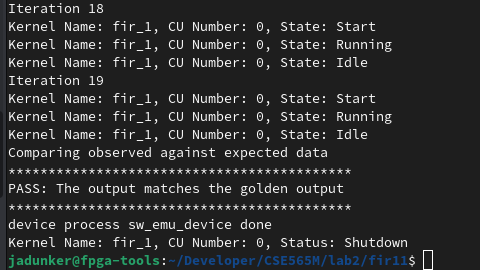
\includegraphics[width=0.8\textwidth]{baseline_sw_emu.png}
        \caption{Software Emulation Output}
        \label{fig:bl_sw_emu_out}
      \end{figure}
      \begin{figure}[h]
        \centering
        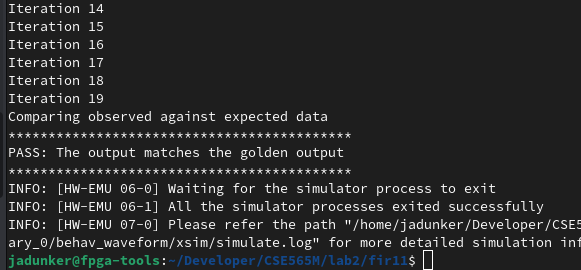
\includegraphics[width=0.8\textwidth]{baseline_hw_emu_2.png}
        \caption{Hardware Emulation Output}
        \label{fig:bl_hw_emu_out}
      \end{figure}
\end{document}